\chapter{Implementation}
In this section will discuss our implementation of AP, The following will be looked at in detail: \begin{itemize}
	\item An overview of the system architecture: How the servers are deployed in the cloud and how they communicate with a client; a breakdown of the components of each server; and potential deployments to be investigated in the future.
	\item Aura Implementation
	\item The algorithms used by the servers to implement AP.
	\item The life cycle of a simulated object as a finite state machine (FSM).
	\item The features and implementation details of the visualiser, including a breakdown of the components of a client and future work to be carried out on the visualiser.
\end{itemize}

\section{System Architecture}
The simulation space is partitioned into regions, with each region consisting of its own instance of PhysX running on a dedicated GPU-enabled machine in the cloud. The boundary between regions is defined as a vertical plane, two-dimensionally dividing the simulation space into one region per server. The network library RakNet is used for all message passing between servers. RakNet ensures messages exhibit best effort and are received in sent order. For the purposes of simplicity, the network tick rate (the rate at which RakNet is updated) is the same as the main update rate (the rate at which the main logic of the program is updated, such as processing user input and handling callbacks from PhysX). This removes the need for the aura calculation to account for an extra time delay between network update and main update.

When objects project auras they are added to a send aura buffer that is sent to all servers associated to the boundary of concern. Each object has a unique identifier (ID). When an aura is received by a server, an aura is created if it does not already exist, otherwise the aura is updated using the data received. When an object is no longer projecting its aura, the ID of that object is added to the delete buffer which is then sent to all servers neighbouring the boundary.

When objects traverse region boundaries, they are added to a migration buffer with all information required to duplicate an object at a neighbouring server. The contents of each migration buffer are sent to the associated server, which will then be responsible for hosting the migrated objects. When migration messages are received, the migrated objects are created within the receiving server's simulation.

Clients connect to all servers and are provided with a streamed visualisation of the simulation in real-time. Clients may also interact with and influence the simulation through client-created replicas and static objects, and RPCs, providing a comprehensive solution for real-time interactive physics. The client system was built using the Unreal Engine. Once a client is connected, the position and states (replicas) of all objects in the simulation are sent from each server to the client via the RakNet Replica Manager.

An overview of the system architecture is illustrated in Fig. \ref{SystemOverview}.

For the implementation of this project, Amazon Web Services (AWS) was selected as the cloud provider, giving access to GPU-enabled instances (G2 instances). The PhysX Samples project (a publicly available project for demonstrating the features and capabilities of PhysX) was used as a starting point for this project, as this was a relatively minimal project that uses PhysX but with some useful features for use in development of this project, such as a basic renderer and many helper methods for using PhysX. For the purposes of automated testing and for running experiments, the testing library, Gtest, was used.

\begin{figure}[t]
	\centering
	\scalebox{1.5}{\input{Figs/OurDeploymentV2.pdf_tex}}
	\caption{Network Topology. Each server is an EC2 instance in the cloud, running our implementation of AP, which includes an instance of PhysX. The client is a local machine running the visualiser built in Unreal Engine. Servers connect to each other in order to exchange messages for aura creation/update and deletion and the migration of objects. The client receives replica updates from each server as well as sending client-created replicas and static objects, and RPCs.}
	\label{SystemOverview}
\end{figure}

\subsection{Server-Region Topology}\label{Topology}
Server-region topologies and how they affect the communication requirements between servers will now be discussed. 
AP allows for the simulation space to be partitioned into any topology. In terms of communication, all servers need to communicate with all of their neighbours in order to satisfy the solution to the corner case, as described in \ref{CornerCase}. We define a neighbour as any server that shares a region boundary, including at a corner. 

The simplest topology that can be used is a column layout, as shown in Fig. \ref{ServerColumnLayout}. In column layout, servers have at most 2 neighbours, this topology therefore has the fewest server connection requirements. It should be noted however, that fewer server connection requirements doesn't necessarily mean less network traffic as the traffic between 2 servers is dependent on the activity of the simulation near the server boundary.

\definecolor{rvwvcq}{rgb}{0.08235294117647059,0.396078431372549,0.7529411764705882}
\definecolor{sim}{rgb}{0,0.2,0.5}

\begin{figure}[!t]	
	\begin{tikzpicture}[line cap=round,line join=round,>=triangle 45,x=1cm,y=1cm,scale=1.5]
	\clip(-2.25,0) rectangle (8.4,3.75);
	\fill[line width=0.8pt,color=sim,fill=sim,fill opacity=0.1] (-2.25,3) -- (-2.25,0) -- (8.25,0) -- (8.25,3) -- cycle;
	\draw (-1.5,3.5) node[anchor=center] {Server 0};
	\draw (1.5,3.5) node[anchor=center] {Server 1};
	\draw (4.5,3.5) node[anchor=center] {\textbf{...}};
	\draw (7.5,3.5) node[anchor=center] {Server N-1};
	\draw [line width=2pt] (0,0)-- (0,3);
	\draw [line width=2pt] (3,0)-- (3,3);
	\draw [line width=2pt] (6,0)-- (6,3);
	\end{tikzpicture}
	\centering
	\begin{tikzpicture}[line cap=round,line join=round,>=triangle 45,x=1cm,y=1cm]
	\clip(-4,0) rectangle (7,1.5);
	\draw [line width=2pt] (-0.5,0.7)-- (-0.3,0.7);
	\draw (-0.1,0.7) node[anchor=west] {Server-Region Boundary};
	\end{tikzpicture}
	\caption{Column Layout}
	\label{ServerColumnLayout}
\end{figure}

Any topology more complex than columns will result in corners being present in the topology. The simplest corner that can exist is between three servers, as shown in Fig. \ref{3ServerCornerLayout}. All three server must communicate when a corner between three servers exists, this is required for the solution to the corner case (as described in \ref{CornerCase}). For example, in  Fig. \ref{3ServerCornerLayout}, a cluster of objects being hosted by server 2 may exist across the boundary between server 0, objects on the edge of the cluster may be positioned deep into server 0's region. In addition a cluster of objects being hosted on server 1 may exist across the boundary between server 1 and server 0 with some objects in the cluster being deep into server 0's region. Without the auras from the server 0 - server 1 boundary being sent to server 2 and vice versa, the two clusters will be unaware of each other's existence. From Server 0's perspective, the two clusters may have overlapping auras, and so should be being simulated on the same server. In order to prevent this, the auras from the boundaries of all neighbours need to be exchanged.

\begin{figure}[!t]
	\begin{subfigure}{.5\textwidth}
		\begin{tikzpicture}[line cap=round,line join=round,>=triangle 45,x=1cm,y=1cm,scale=1.2]
		\fill[line width=0.8pt,color=sim,fill=sim,fill opacity=0.1] (-3,3) -- (-3,-2) -- (3,-2) -- (3,3) -- cycle;
		\draw [line width=2pt] (-3,0)-- (3,0);
		\draw [line width=2pt] (0,3)-- (0,0);
		\draw (-1.5,2.5) node[anchor=center] {Server 0};
		\draw (1.5,2.5) node[anchor=center] {Server 1};
		\draw (0,-1) node[anchor=center] {Server 2};
		\end{tikzpicture}
		\centering
		\begin{tikzpicture}[line cap=round,line join=round,>=triangle 45,x=1cm,y=1cm]
		\draw [line width=2pt] (-2.5,0.5)-- (-2.3,0.5);
		\draw (-2.1,0.5) node[anchor=west] {Region Boundary};
		\end{tikzpicture}
		\caption{3 Server Corner Topology}
		\label{3ServerCornerLayout}
	\end{subfigure}%
	\begin{subfigure}{.5\textwidth}
		\begin{tikzpicture}[line cap=round,line join=round,>=triangle 45,x=1cm,y=1cm,scale=1.2]
		%	\clip(-3,-3) rectangle (3,3);
		\fill[line width=0.8pt,color=sim,fill=sim,fill opacity=0.1] (-3,3) -- (-3,-3) -- (3,-3) -- (3,3) -- cycle;
		\draw [line width=2pt] (-3,0)-- (3,0);
		\draw [line width=2pt] (0,3)-- (0,0);
		\draw (-1.5,2.5) node[anchor=center] {Server 0};
		\draw (1.5,2.5) node[anchor=center] {Server 1};
		\draw (-1.5,-2.5) node[anchor=center] {Server 2};
		\draw (1.5,-2.5) node[anchor=center] {Server 3};
		\draw [line width=2pt] (0,0)-- (0,-3);
		\end{tikzpicture}
		\centering
		\caption{4 Server Corner Topology}
		\label{4ServerCornerLayout}
	\end{subfigure}
	\caption{Corner Layouts}
	\label{ServerCornerLayout}
\end{figure}

An example of a topology that includes corners with no more than 3 servers neighbouring is illustrated in Fig. \ref{BrickLayout}. In this topology, the maximum number of server connections required would be 6, as server 3 has 6 neighbouring servers. It should be noted that not all servers need to communicate with each other, for example server 0 does not neighbour with servers 4 or 6, so no communication is needed.

\begin{figure}[!t]	
	\begin{tikzpicture}[line cap=round,line join=round,>=triangle 45,x=1cm,y=1cm,scale=0.875]
		\fill[line width=0.8pt,color=sim,fill=sim,fill opacity=0.1] (-6,-9) -- (-6,0) -- (12,0) -- (12,-9) -- cycle;
		\draw [line width=2pt] (-3,-3)-- (3,-3);
		\draw [line width=2pt] (-3,-3)-- (-3,0);
		\draw [line width=2pt] (-3,0)-- (3,0);
		\draw [line width=2pt] (3,0)-- (3,-3);
		\draw [line width=2pt] (-6,-6)-- (0,-6);
		\draw [line width=2pt] (-6,-6)-- (-6,-3);
		\draw [line width=2pt] (-6,-3)-- (0,-3);
		\draw [line width=2pt] (0,-3)-- (0,-6);
		\draw [line width=2pt] (0,-6)-- (6,-6);
		\draw [line width=2pt] (0,-6)-- (0,-3);
		\draw [line width=2pt] (0,-3)-- (6,-3);
		\draw [line width=2pt] (6,-3)-- (6,-6);
		\draw [line width=2pt] (3,-3)-- (9,-3);
		\draw [line width=2pt] (3,-3)-- (3,0);
		\draw [line width=2pt] (3,0)-- (9,0);
		\draw [line width=2pt] (9,0)-- (9,-3);
		\draw [line width=2pt] (6,-6)-- (12,-6);
		\draw [line width=2pt] (6,-6)-- (6,-3);
		\draw [line width=2pt] (6,-3)-- (12,-3);
		\draw [line width=2pt] (12,-3)-- (12,-6);
		\draw [line width=2pt] (-3,-9)-- (3,-9);
		\draw [line width=2pt] (-3,-9)-- (-3,-6);
		\draw [line width=2pt] (-3,-6)-- (3,-6);
		\draw [line width=2pt] (3,-6)-- (3,-9);
		\draw [line width=2pt] (3,-9)-- (9,-9);
		\draw [line width=2pt] (3,-9)-- (3,-6);
		\draw [line width=2pt] (3,-6)-- (9,-6);
		\draw [line width=2pt] (9,-6)-- (9,-9);
		\draw (0.0,-1.5) node[anchor=center] {Server 0};
		\draw (6,-1.5) node[anchor=center] {Server 1};
		\draw (-3,-4.5) node[anchor=center] {Server 2};
		\draw (3,-4.5) node[anchor=center] {Server 3};
		\draw (9,-4.5) node[anchor=center] {Server 4};
		\draw (0,-7.5) node[anchor=center] {Server 5};
		\draw (6,-7.5) node[anchor=center] {Server 6};
	\end{tikzpicture}
	\centering
	\begin{tikzpicture}[line cap=round,line join=round,>=triangle 45,x=1cm,y=1cm]
	\clip(-4,0) rectangle (7,1.5);
	\draw [line width=2pt] (-0.5,0.7)-- (-0.3,0.7);
	\draw (-0.1,0.7) node[anchor=west] {Server-Region Boundary};
	\end{tikzpicture}
	\caption{An example topology using only 3-server corners}
	\label{BrickLayout}
\end{figure}

An example of a topology that uses 4-server corners is illustrated in Fig. \ref{GridLayout}. In this topology the maximum number of server connections required would be 8, as server 4 has 8 neighbouring nodes. It should be noted that not all servers need to communicate with each other, for example server 0 does not need to communicate with servers 2 or 5 as they are not neighbouring servers.

\begin{figure}[!t]
	\begin{tikzpicture}[line cap=round,line join=round,>=triangle 45,x=1cm,y=1cm]
	\fill[line width=0.8pt,color=sim,fill=sim,fill opacity=0.1] (-3,3) -- (-3,-6) -- (6,-6) -- (6,3) -- cycle;
	\draw [line width=2pt] (-3,0)-- (6,0);
	\draw [line width=2pt] (0,3)-- (0,-6);
	\draw [line width=2pt] (-3,-3)-- (6,-3);
	\draw [line width=2pt] (3,3)-- (3,-6);
	\draw (-1.5,1.5) node[anchor=center] {Server 0};
	\draw (1.5,1.5) node[anchor=center] {Server 1};
	\draw (4.5,1.5) node[anchor=center] {Server 2};
	\draw (-1.5,-1.5) node[anchor=center] {Server 3};
	\draw (1.5,-1.5) node[anchor=center] {Server 4};
	\draw (4.5,-1.5) node[anchor=center] {Server 5};
	\draw (-1.5,-4.5) node[anchor=center] {Server 6};
	\draw (1.5,-4.5) node[anchor=center] {Server 7};
	\draw (4.5,-4.5) node[anchor=center] {Server 8};
	\end{tikzpicture}
	\centering
	\begin{tikzpicture}[line cap=round,line join=round,>=triangle 45,x=1cm,y=1cm]
	\clip(-4,0) rectangle (7,1.5);
	\draw [line width=2pt] (-0.5,0.7)-- (-0.3,0.7);
	\draw (-0.1,0.7) node[anchor=west] {Server-Region Boundary};
	\end{tikzpicture}
	\caption{An example topology using 4-server corners}
	\label{GridLayout}
\end{figure}

%TODO: Talk about adaptive server boundaries in the future. Talk about assumptions that clusters do not cross width between nodes and how adaptive boundaries could lead to this

\subsection{Individual Server Breakdown}
The components that make up an individual server, as illustrated in \ref{fig_stack}, will now be discussed. Each server is connected to the client ($C_1$) and all neighbouring servers $S_1..S_N$ (the definition of neighbouring nodes is discussed in \ref{Topology}). The server connects to both of these types through the RakNet library. RakNet includes the Replica Manager and RPCs used by client. 

For each boundary with a neighbouring server, a server has three message buffers 1) A migration buffer for sending objects to the server corresponding with that boundary. Each element in the buffer is a message for one object migration. Each migration message contains all data necessary to reproduce the object on the receiving server. 2) An aura creation/update buffer, each element of the buffer is a message for the creation or update of an aura and includes ID, position and radius of the aura. The contents of this buffer are sent to all neighbouring servers, not just the server corresponding with this boundary. The messages structure for both creation and update are identical as the receiving server creates a new aura if one does not already exist for the corresponding object (determined using the ID), otherwise the message is just used to update the state of the existing aura. 3) An aura delete buffer, each element of the buffer is a message for the deletion of an aura, which consists of the aura's ID. The contents of this buffer are sent to all neighbouring servers, not just the server corresponding with this boundary.

Aura Projection receives and processes the messages received from the neighbouring servers. This includes the creation of migrating objects in the PhysX simulation, the creation and updates of the trigger volumes for auras and the deletion of auras in the PhysX simulation.

PhysX provides callbacks for collision events, such as when an object collides with an object's aura or collides with a trigger boundary aura.

The Replica manager tracks the states of objects that are being replicated and sends changes of state to the client. The Replica manager also receives replica creation messages from the client (as described in \ref{Client-CreatedReplicas})

RPCs allow the client to call procedures on the server, including the creation of server-created replicas (as described in \ref{Server-CreatedReplicas}). RPCs enable the client to interact with the servers through various features described in \ref{Interactivity}

\begin{figure}[t]
	\centering
	\resizebox{\linewidth}{!}{\input{Figs/Architecture.pdf_tex}}
	%\scalebox{1.1}{\input{Figs/Architecture.pdf_tex}}
	\caption{Server Breakdown. This diagram shows a breakdown of the components of an individual server.}
	\label{fig_stack}
\end{figure}

\subsection{Future Architecture}
System architectures which could be investigated in the future will now be proposed and discussed. A limitation of the current architecture is that a client must connect to all servers; servers that are responsible for running the simulation also have the overhead of connecting to many clients. An alternative to this is to make the use of an `overseer' node, which acts as a middle-man for communication with all the servers, as illustrated in Fig. \ref{OverseerNode}. The overseer node is co-located in the cloud with the simulation servers. The clients all connect to the overseer node, but all the servers only connect to one overseer node, reducing the overhead of many clients connecting to a server, freeing up computational resources on each simulation server, allowing more resources to be used for the simulation itself. An additional advantage of this approach is it allows for some fault-tolerance. If one or more simulation servers were to fail, the overseer node has a copy of the states of all objects from those servers, meaning those spatial partitions of the simulation could be restored. The disadvantage of using an overseer node is the additional latency between client and simulation server, messages now have to be processed by the overseer node between the simulation servers and clients. For example, if a replicated object moves in one of the simulation servers, the update message for that object has to be processed and sent by the simulation server, sent over the network to the overseer, received and processed by the overseer node and then sent over the network to all connected clients. The additional latency is due to the communication latency between simulation server and overseer node and the time taken to process messages on the overseer node.

\begin{figure}
	\centering
	\scalebox{1.25}{\input{Figs/OverseerNode.pdf_tex}}
	\caption{Overseer node.}
	\label{OverseerNode}
\end{figure}

The limitation of the use of an overseer node is the number of clients that can connect is limited to the amount that can be handled by a single overseer node. In order to enable a scalable number of clients, multiple overseer nodes could be employed, dividing the workload between overseer nodes, allowing for many more clients to connect. This is illustrated in \ref{MultiOverseer}.

\begin{figure}
	\centering
	\scalebox{1.25}{\input{Figs/MultipleOverseerNodes.pdf_tex}}
	\caption{Multiple overseer nodes for scalable number of clients.}
	\label{MultiOverseer}
\end{figure}

\begin{figure}
	\centering
	\scalebox{1.25}{\input{Figs/EdgeBasedOverseerNodes.pdf_tex}}
	\caption{Edge-based overseer nodes.}
\end{figure}

In the current system architecture, the rendering work is carried out on the client machine. An alternative to this is to have the rendering performed on dedicated render nodes in the cloud, as illustrated in \ref{RenderNodes}. The results video could then be streamed to clients. This has the advantage of enabling low computational power devices, such as mobile devices, to display higher quality graphics, beyond what would be achievable on low computational power devices. Additionally, it means there is very low latency between the physics simulation and the renderer, meaning what is displayed is closer to the actual current state of the physics simulation. The disadvantage of this approach is the latency time between the client and the renderer.

%TODO: Give example of long latency between client and renderer. Talk about other disadvantages, more computational workload in cloud. Compare workload of video streaming to streaming replicas.

\begin{figure}
	\centering
	\scalebox{1.25}{\input{Figs/DedicatedRenderNodes.pdf_tex}}
	\caption{Dedicated render nodes in cloud.}
	\label{RenderNodes}
\end{figure}

\begin{figure}
	\centering
	\scalebox{1.25}{\input{Figs/EdgeBasedRenderNodes.pdf_tex}}
	\caption{Dedicated render nodes in edge.}
\end{figure}

\section{Aura Implementation}
How the auras in AP are implemented will now be described at a high-level, before a formal description of the algorithms using pseudo-code is given in \ref{Algorithms}.
Auras are implemented through the use of trigger volumes (non-physically interacting volumes, that generate trigger collision callbacks). Two trigger volumes are used for different purposes. 
The first is used for auras that are being received from remote servers. When an aura is received, a trigger volume, consisting of a sphere, is created at the corresponding position with a given radius. The second trigger volume used is by the server-region boundaries. Each server-region boundary has a trigger volume that extends inside the server's region, it extends the same distance as the aura radius, minus the bounding sphere of an object. This is used to determine when an object should begin and stop having its aura sent to neighbouring servers and avoid the need for per-object checks for proximity to the server-region boundary. When an object collides with the aura trigger boundary, the aura begins being sent, when an object leaves the aura trigger boundary, an aura delete message is sent.
Each server-region boundary has a trigger volume, objects may collide with multiple aura trigger boundaries, meaning auras can be sent to multiple servers, as illustrated in Fig. \ref{AuraCorner}.
%TODO: Boundary has a trigger volume, illustrate with diagram. Is this mentioned elsewhere?

It should be noted that an object's bounding sphere may be intersecting the boundary trigger, but the object itself may not, resulting in no aura being broadcast. However, this will not lead to problems with auras not being broadcast when a possible interaction could occur, as the bounding sphere is a simplification used for the aura. Using the actual shape of the object to determine when to begin broadcasting the aura is more accurate than the bounding sphere simplification.

When a server begins communicating an aura, a message is added to the aura creation/update buffer. This message consists of the position of the centre of the aura, the radius of the aura. % and a flag signifying whether or not this is a creation message or not. Flag is not currently used as often causes issue in the corner case, possibly due to multiple types of messages concerncing one object being sent and recieved in the same tick.
The contents of the buffer are then broadcast to all neighbouring servers. When aura creation/update messages are received and an aura for that object does not already exist, a new aura, a sphere trigger volume, is created at that position with the given radius.
Whenever an object projecting an aura moves, and update message is added to the aura creation/update buffer, containing the new position and radius of the aura (aura radius is currently fixed, but may become dynamic in the future). The contents of the buffer are broadcast to all neighbouring servers. When the message is received, the positions of the auras are updated. 
If an object leaves aura trigger boundary, either by moving away from the boundary or by being migrated to another server, a delete aura message is added to the aura delete buffer. The contents of the buffer are then broadcast to all neighbouring servers. When the message received, the aura trigger volume is removed from the simulation.

When objects collide with an aura trigger volume from an object on a remote server, a callback from PhysX is generated, when processed by AP, the colliding object is added to the migration buffer for the server the aura is being sent from. In addition, a recursive search is carried out to identify all objects within the cluster (a group of objects with overlapping auras). The entire cluster is added to the migration buffer, so that all objects in the cluster are migrated at once. The contents of the buffer are then sent to the corresponding server.

In addition to auras existing as trigger volumes representing auras of remote objects, servers also track the auras of objects that they are hosting, that are having their auras broadcast. These are used to determine clusters of objects, so that clusters of objects are migrated together, at the same time. When an object begins broadcasting an aura, a query-only shape is attached to the object, which represents the object's aura. When an object is a migration candidate, a scene query is carried out, using this query-only shape, to determine which auras overlap the migration candidate's aura. Using a recursive search, involving a scene query for each object found from the prior query, it is possible to determine the objects in the cluster. If the entire cluster is outside of the host server's region, the entire cluster is added to the migration buffer and sent to the server in which the cluster resides. If any object in the cluster is still within the host server's region, no migration takes place. This prevents clusters being repeatedly being migrated back and forth between servers.

%TODO: Talk about edge-cases of multiple types of messages being sent in on tick.

\begin{figure}
	\centering
	\scalebox{0.75}{\input{Figs/AuraCorner.pdf_tex}}
	\caption{Aura Projection at a 3-way corner intersection. When an object collides with a server aura trigger boundary, the aura begins being sent to the corresponding neighbouring server. In this scenario, an object from server 0 is colliding with two aura trigger boundaries from servers 1 and 2, meaning the aura is sent to both servers 1 and 2. $x$ is the aura distance beyond the boundary sphere of an object and the distance used by the aura trigger boundaries.}
	\label{AuraCorner}
\end{figure}

\section{Algorithms}\label{Algorithms}
$AC$ is called when an object collides with an aura. A recursive search is performed in order to find all objects that would lie within each object's aura, preventing thrashing as discussed in \ref{Thrashing}. Once the recursive search is complete, all objects are added to the send buffer.

\renewcommand{\algorithmicforall}{\textbf{for each}}
\algnewcommand{\LeftComment}[1]{\State \(\triangleright\) #1}
\algnewcommand\And{\textbf{and}}
\algnewcommand\Or{\textbf{or}}

\begin{algorithm}
	\caption{Object Migrate - Aura Collision ($AC$)}\label{auraAlgorithm}
	\begin{algorithmic}[1]
		\Procedure{OnAuraEnter}{}	\Comment{A callback on an object}
		\LeftComment{Track visited objects to prevent infinite recursion}
		\State $\textit{visited := \{\}}$
		\LeftComment{Recursively send object with objects that would lie within each object's aura}
		\State \Call{SendWithOverlaps}{$\textit{thisObject, visited}$}
		\EndProcedure
		\State
		\Procedure{SendWithOverlaps}{$\textit{object, visited}$}
		\LeftComment{Get objects whose auras overlap this object's aura} %using a $\mathcal{O}(n)$ scene query
		\State $\textit{overlaps :=}$ \Call{GetAuraOverlaps}{$\textit{object}$} %\Comment{$\mathcal{O}(n)$ scene query}
		\State
		\ForAll{{$\textit{object} \in \textit{overlaps}$}} :
		\If {$\textit{object} \not \in \textit{visited}$}:
		\State $\textit{visited := visited + object}$
		\State \Call{SendWithOverlaps}{$\textit{object, visited}$}
		\EndIf
		\EndFor
		\State
		\State\Call{AddToSendBuffer}{object}
		\EndProcedure
	\end{algorithmic}
\end{algorithm}

$BT$ is called when an object traverses a boundary. In order to prevent `islands' forming (for example Objects H, I and J in Fig. \ref{AuraProj}), a recursive search is carried out to determine is an object is part of an island or not. If an object is found to not be part of an island, the entire cluster of objects is added to the send buffer, otherwise no action is taken.

\begin{algorithm}
	\caption{Object Migrate - Boundary Traverse ($BT$)}\label{boundaryAlgorithm}
	\begin{algorithmic}[1]	
		\LeftComment{Update called on each boundary}
		\Procedure{BoundaryUpdate}{}
		\State $\textit{checked := \{\}}$	\Comment{Used to prevent duplicate checks}
		\State
		\LeftComment{Loop over fully traversed objects from latest update}
		\ForAll{{$\textit{object} \in \textit{traversed}$}} : 
		%\If {$\textit{object.isSleeping} = \textit{false} \And \textit{object} \not \in \textit{checked}$}:
		\If {$\textit{object} \in \textit{checked}$}:
		\State $\textit{continue}$
		\EndIf
		
		\State $\textit{island := \{\}}$
		\State $\textit{isIsland := }\Call{IslandQuery}{\textit{object, island}}$
		\LeftComment{IslandQuery() returns true if object is part of an island and a list of objects in the island}
		\If {$\textit{isIsland} = \textit{true}$}:
		\State \Call{SendGroup}{$\textit{island}$}
		\EndIf
		\State $\textit{checked := checked + island}$
		\EndFor
		%		\State $\textit{visited := \{\}}$	\Comment{Track visited to prevent infinite recursion}
		%		\State \Call{SendWithOverlaps}{$\textit{thisObject, visited}$}
		\EndProcedure
		\State
		\Function{IslandQuery}{$\textit{object, visited}$}
		\State $\textit{visited := visited + object}$
		\If {$\textit{object.overlapsHostRegion = true}$}
		\State return $\textit{false}$
		\EndIf
		%\If {$\textit{object.boundaryCollisionCount = 0}$}
		%\State return $\textit{false}$
		%\EndIf
		\State
		\LeftComment{Get objects whose auras overlap this object's aura} %using a $\mathcal{O}(n)$ scene query
		\State $\textit{overlaps :=}$ \Call{GetMutalAuraOverlaps}{$\textit{object}$}
		\State
		\LeftComment{If all objects with overlapping auras are islands, then this object is an island}
		\State $\textit{isIsland := true}$
		\ForAll{{$\textit{object} \in \textit{overlaps}$}} :
		\If {$\textit{object} \not \in \textit{visited}$}:
		\State $\textit{isIsland \&= }$ \Call{IslandQuery}{$\textit{object,visited}$}
		\EndIf
		\EndFor
		\State return $\textit{isIsland}$
		\EndFunction
		%		
		%		\Procedure{SendWithOverlaps}{$\textit{object, visited}$}
		%		\State $\textit{overlaps :=}$ \Call{GetOverlaps}{$\textit{object}$} \Comment{$\mathcal{O}(n)$ scene query}
		%		\ForAll{{$\textit{object} \in \textit{overlaps}$}} :
		%		\If {$\textit{object} \not \in \textit{visited}$}:
		%		\State $\textit{visited := visited + object}$
		%		\State \Call{SendWithOverlaps}{$\textit{object, visited}$}
		%		\EndIf
		%		\EndFor
		%		
		%		\State\Call{Send}{object}
		%		\EndProcedure
	\end{algorithmic}
\end{algorithm}

$OBC$ is called when an object collides with a boundary. The object's aura is calculated and added to the boundary's send aura buffer. A host aura is also created, to allow for the checking of mutual aura overlaps and prevent thrashing, if this is the first boundary intersection.

\begin{algorithm}
	\caption{Create Aura - Object boundary collision ($OBC$)}\label{createAuraBoundaryAlgorithm}
	\begin{algorithmic}[1]
		\LeftComment{A callback on an object, called when an object collides with a boundary}
		\Procedure{OnBoundaryEnter}{$\textit{boundary}$}
		\State \Call{AddToAuraBuffer}{$\textit{boundary, this}$}
		\State
		\LeftComment{Create `host aura' so GetMutalAuraOverlaps() will detect this object's aura}
		\If {$\textit{boundaryIntersections = 0}$}
		\State \Call{CreateHostAura}{$\textit{}$}
		\EndIf
		\State $\textit{boundaryIntersections := boundaryIntersections + 1}$
		%\State $\textit{boundariesEntered := boundariesEntered + boundary}$
		%	\State $\textit{boundary->addToOverlappingOtherObjects(m_rigidDynamic)}$
		%	\State $\textit{boundary->addBoundaryBodyToSendBuffer(this)}$
		\EndProcedure
	\end{algorithmic}
\end{algorithm}

$OBU$ is called once per frame that an object is intersecting a boundary. If the object is not `sleeping', a new aura is calculated and added to the boundary's send buffer and the host aura is updated.

The isSleeping() function returns true if an object is sleeping. From the PhysX documentation:
An object is considered `sleeping' when an actor does not move for a period of time. (The default PhysX period of time is $0.4s$ and this is the value used in our approach). Objects are `woken up' when they are touched by an awake object. 

\begin{algorithm}
	\caption{Update Aura - Object boundary update ($OBU$)}\label{objectWithAuraAlgorithm}
	\begin{algorithmic}[1]
		\LeftComment{A callback on an object, called per step per boundary the object is colliding with}
		\Procedure{onBoundaryUpdate}{$\textit{boundary}$}
		\If {$\textit{this.isSleeping = true}$}
		\State $\textit{return}$
		\EndIf
		\LeftComment{Send Aura Delta}
		\State \Call{AddToAuraBuffer}{$\textit{boundary, this}$} 
		\State \Call{UpdateHostAura}{$\textit{}$}
		%		if (!m_hasBeenSent 
		%	&& (m_app->isBoundaryOtherActor(triggerPair.triggerActor))
		%	&& !m_rigidDynamic->isSleeping()
		%	&& !m_rigidDynamic->getAngularVelocity().isZero()
		%	&& !m_rigidDynamic->getLinearVelocity().isZero()
		%	)
		%	{
		%		OrionBoundaryOther* boundary = (OrionBoundaryOther*)triggerPair.triggerActor->userData;
		%		boundary->addBoundaryBodyToSendBuffer(this);
		%	}
		%	
		%	if (m_app->isBoundaryOtherActor(triggerPair.triggerActor))
		%	{
		%		updateBoundingBox();
		%	}
		\EndProcedure
	\end{algorithmic}
\end{algorithm}

$OBE$ is called when an object is no longer intersecting a boundary. The object is added to the boundary's remove aura buffer. If the object is no longer intersecting any boundaries, the host aura is deleted.

\begin{algorithm}
	\caption{Destroy Aura - Object boundary exit ($OBE$)}\label{destroyAuraAlgorithm}
	\begin{algorithmic}[1]
		\LeftComment{A callback on an object, called when an object exits a boundary}
		\Procedure{onBoundaryExit}{$\textit{boundary}$}
		\State \Call{AddtoDeleteAuraBuffer}{$\textit{}$}
		\State
		\LeftComment{If object is no longer sending an aura, no need to keep a `host aura'}
		\State $\textit{boundaryIntersections := boundaryIntersections - 1}$
		\If {$\textit{boundaryIntersections = 0}$}
		\State \Call{DeleteHostAura}{$\textit{}$}
		\EndIf
		
		%	// If leaving boundary of other simulation, send message removing object from other boundary triggers
		%	if (!m_hasBeenSent && m_app->isBoundaryOtherActor(triggerPair.triggerActor))
		%	{
		%		OrionBoundaryOther* boundary = (OrionBoundaryOther*)triggerPair.triggerActor->userData;
		%		vector<OrionBoundaryOther*>::iterator found = find(m_boundariesWithAuras.begin(), m_boundariesWithAuras.end(), boundary);
		%		if (found != m_boundariesWithAuras.end())
		%		{
		%			boundary->addBoundaryBodyRemoveToSendBuffer(m_index);
		%			boundary->removeFromOverlappingOtherObjects(m_rigidDynamic);
		%			m_boundariesWithAuras.erase(find(m_boundariesWithAuras.begin(), m_boundariesWithAuras.end(), boundary));
		%		}
		%	}
		%	
		%	if (m_app->isBoundaryOtherActor(triggerPair.triggerActor))
		%	{
		%		m_partiallyInsideOtherCount--;
		%		PX_ASSERT(m_partiallyInsideOtherCount >= 0);
		%		if (m_partiallyInsideOtherCount == 0)
		%		{
		%			deleteBoundingBox();
		%		}
		%	}
		\EndProcedure
	\end{algorithmic}
\end{algorithm}

$BNU$ is called once per network connection between servers. It is responsible for sending and receiving object migrations and auras between servers, including the sending and receiving of auras from boundaries between other neighbouring remote servers.

\begin{algorithm}
	\caption{Boundary Network Update ($BNU$)}\label{boundaryNetworkAlgorithm}
	\begin{algorithmic}[1]
		\LeftComment{Update called once per network connection}
		\Procedure{Network Update}{}
		\LeftComment{Exchange migrations with target server}
		\State \Call{SendObjectsInBuffer}{}
		\State \Call{ReceiveObjects}{}
		\State
		\LeftComment{Send aura state updates to all neighbours}
		\ForAll{{$\textit{neighbour} \in \textit{neighbours}$}} :
		\State \Call{SendAurasInBuffer}{}
		\State \Call{SendDeleteAurasInBuffer}{}
		\State \Call{ReceiveAuras}{}
		\State \Call{ReceiveDeleteAuras}{}
		\EndFor
		%	sendRigidDynamics();
		%recvRigidDynamicUpdate();
		%
		%vector<OrionAuraExchangeBoundary*>::const_iterator it;
		%for (it = m_auraExchange.begin(); it != m_auraExchange.end(); ++it)
		%{
		%	sendBoundaryBodies(*it);
		%	sendBoundaryBodiesRemove(*it);
		%	recvBoundaryBodyUpdate(*it);
		%	recvBoundaryBodyRemoveUpdate(*it);
		%}
		\EndProcedure
	\end{algorithmic}
\end{algorithm}

\section{FSM}
We will now discuss the state of an object in the context of AP, i.e. not position and rotation of an object, but the state of object as it is being treated by AP.

An object has two entry states, it is either received from another server via the network or it is injected into the simulation. Immediately the object's position determines its next state. If the object is not intersecting a server boundary and is not colliding with an aura, the object moves into the Host Region state. If the object is intersecting a sever boundary, it moves into the intersecting boundary state. If the object is outside of the server's region, such as is if the object is injected into a server at position the server is not responsible for, the object changes states to the boundary traversed state.
%TODO: Remaning states and transitions

\begin{figure}[hbt]
	\centering
	\resizebox{\columnwidth}{!}{
		\begin{tikzpicture}[>=stealth',shorten >=1pt,auto,node distance=2.5cm]
		\node[initial,state,accepting,align=center] (R) {$Receive$};
		\node[initial,state,accepting] (S) [below of=R] {$Inject$};
		\node[state]         (q2) [below of=S, node distance=3cm, text width=2cm, align=center] {$Intersecting$ $Boundary$};
		\node[state]         (q1) [left of=q2, node distance=4cm]  {$Host$ $Region$};
		\node[state]         (q3) [right of=q2, node distance=4cm, text width=2cm, align=center] {$Boundary$ $Traversed$};
		\node[state]         (q4) [below of=q2, node distance=4cm] {$Sent$};
		\node[state]         (q5) [right of=q4] {$Destroyed$};
		
		
		\path[->] 
		(R) edge node {} (S)
		(S) edge [bend right] node [left, text width=2cm, align=center] {No Collision} (q1)
		(S) edge node [anchor=center, text width=1.5cm, align=left] {$OBC$} (q2)
		(S) edge [bend left] node [right, text width=2cm, align=center] {Outside Owner} (q3)
		%(q1) edge [loop above] node {} (q1)
		%(q2) edge [loop left] node {} (q2)
		(q3) edge [loop below] node [above] {$BT$} (q3)
		(q1) edge node [left, text width=2cm, align=center] {$AC$} (q4)
		(q2) edge node [anchor=center, text width=2cm, align=center] {$AC$} (q4)
		(q3) edge node [anchor=center, text width=2cm, align=center] {$BT$/$AC$} (q4)
		
		(q1) edge [bend left] node [anchor=center, text width=1.5cm, align=center, above] {$OBC$} (q2)
		(q2) edge [bend left] node [anchor=center, text width=2cm, align=center, above] {$OBE$} (q1)
		(q3) edge [bend left] node [anchor=center, text width=2cm, align=center] {Owner Collision} (q2)
		(q2) edge [bend left] node [anchor=center, above, text width=2cm, align=center] {Owner Exit} (q3)
		
		(q4) edge node {} (q5)
		
		%(S)  edge [loop above] node {a} (S)
		%edge              node {a} (q1)
		%(q1) edge [bend left]  node {a} (S)
		%edge              node {b} (q2)
		%(q2) edge [loop above] node {b} (q2)
		%edge [bend left]  node {b} (q1)
		;
		\end{tikzpicture}
	}
\end{figure}

\section{The Visualiser}
%We discuss the features and implementation of the visualiser, including server and client created replicas, static objects and interactivity. The challenges of multiple servers are explained and our solutions justified. Screenshots from demo scenes have been included.
We will now discuss the details of the visualiser, both the features and implementation details.

The visualiser is built using Unreal Engine and the RakNet plugin.

%TODO: Add client-created server regions feature

\begin{figure}[!t]
	\centering
	\includegraphics[width=\textwidth]{Blocks}
	\caption{Stacks of objects near and on a corner boundary. This demo scene consists of two large stacks of server created cuboid replicas near the corner of four server regions. Either side of each server boundary are random injection volumes, in which server created objects are injected into the simulation, randomly, within a volume. Each colour represents a different owning server.}
	\label{fig_screen1}
\end{figure}

\begin{figure}[!t]
	\centering
	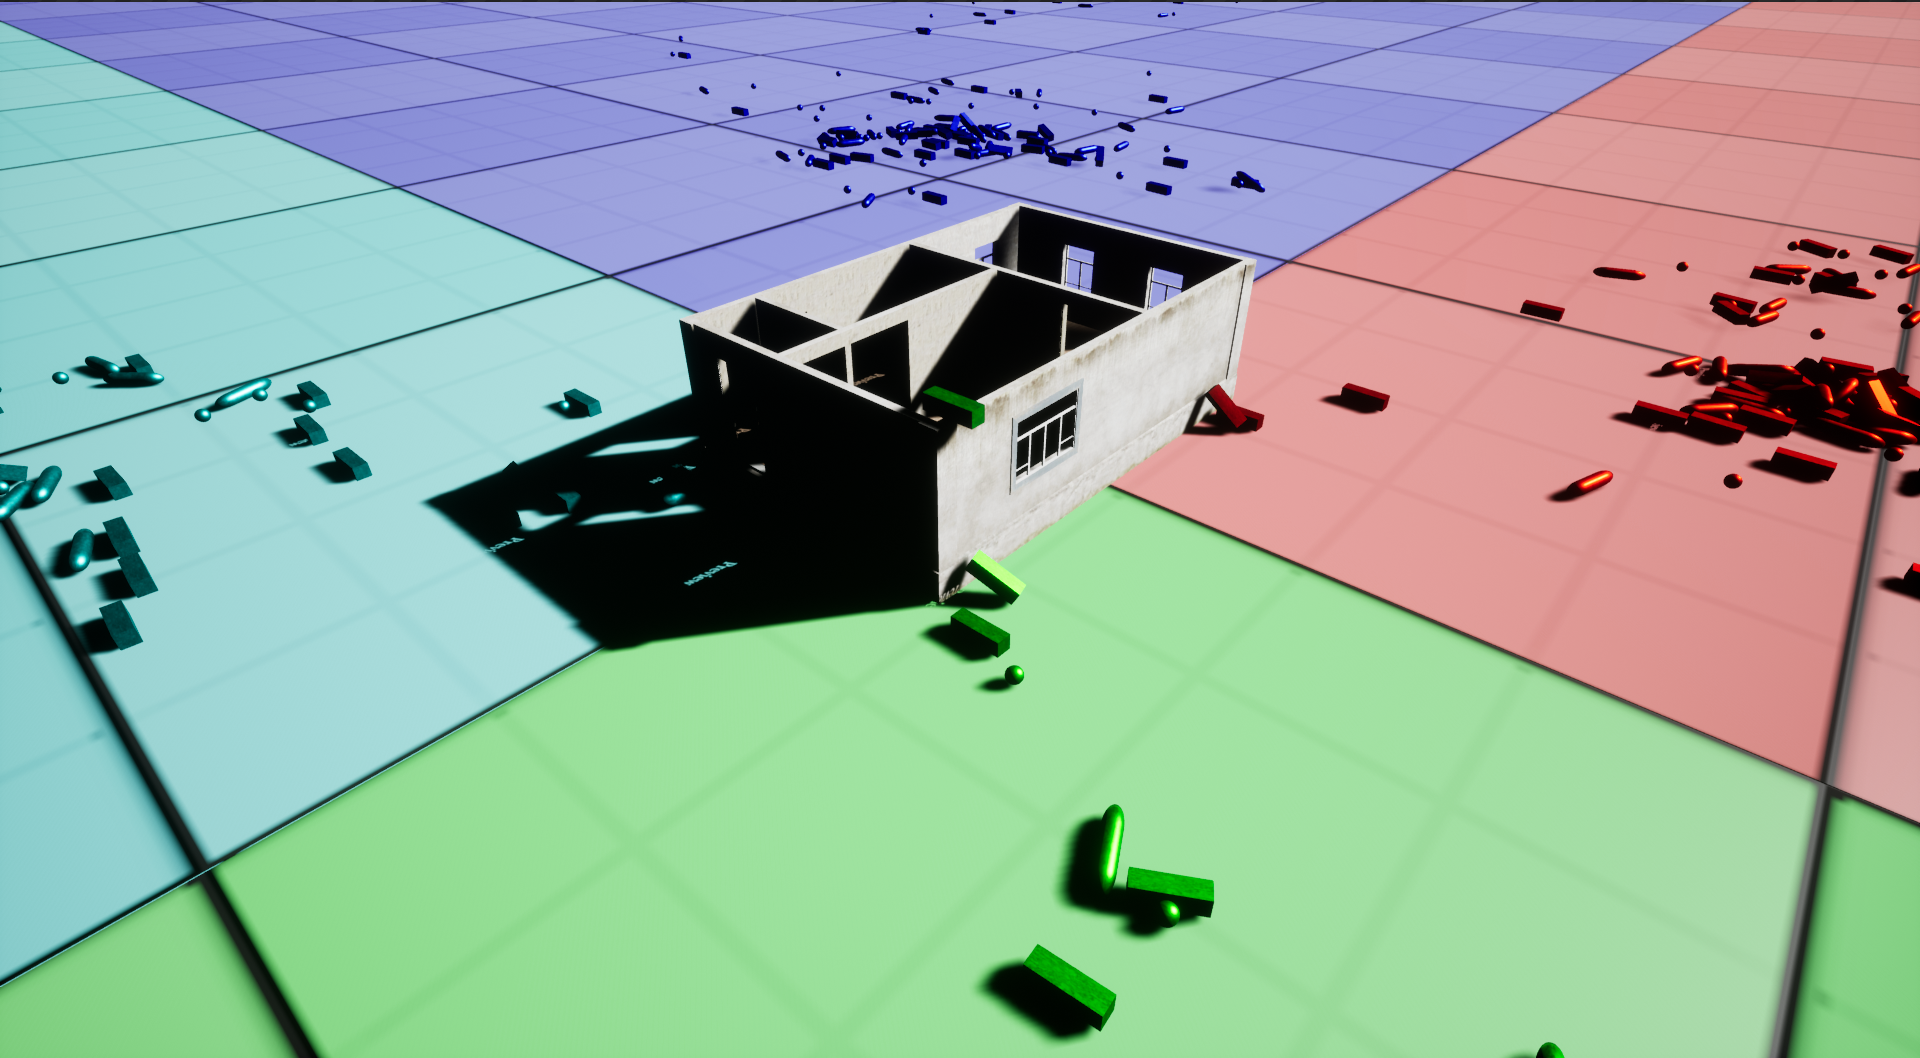
\includegraphics[width=\textwidth]{screenshot}
	\caption{A static object on a corner boundary surrounded by objects being simulated on different servers. This demo scene includes a client-created static object (a building), which is being simulated on all servers. Numerous server created objects surround the building, which have been triggered from within the client.}
	\label{fig_screen2}
\end{figure}

\subsection{Terminology}
Before discussing specific details of the visualiser, we must first define terms used.
\begin{itemize}
	\item The visualiser: The software application that is capable of connecting to AP servers and display replicas of objects on the servers.
	\item The editor: This refers to the Unreal Engine Editor. The version of the editor used for the visualiser is UE4.19.2
	\item Edit-time: When scenes are being edited in the Unreal Engine Editor, before the visualiser has been packaged.
	\item Run-time: When the visualiser is running
	\item Player: The in-visualiser representation of the user. Has a position and rotation. The camera for rendering is attached to the player
	\item Replica object: A representation displayed in the visualiser of an object being simulated on a server, which is intended to replicate the physical state of the object on the server.
\end{itemize}

\subsection{Overview}
The visualiser connects to multiple servers, objects are simulated on server and those objects from all servers are replicated on the visualiser. These are referred to as replica objects. The visualiser uses RakNet's ReplicaManager, which is responsible for: the creation of replicas objects on both the server and client; communicating the state of objects from the server to the client, in order for the replica objects to be replicated; and the deletion of replica objects. Replica objects are replicated on the visualiser by the server sending the state (position, rotation) to the client, the replica representation on the client is then updated with the newly received state from the server. The object state is optimised to reduce processing and network overhead, by only sending updates of the position and rotation to the client, when they change on the server. In the visualiser, replica objects are kinematic objects, i.e. they are not physically simulated in the visualiser, their physical states are updated entirely by messages received from the server, such as their movement from velocity and no interactions, such as collisions are simulated in the visualiser.

Replica objects can be created in one of two ways. Either by the server or by the client. We will now discuss the implementation details of each type of replica creation.

\subsection{Server-created replica objects}\label{Server-CreatedReplicas}
The visualiser supports server-created replica objects, which are limited to pre-defined basic objects (cuboid, sphere \& capsule). A different render material per server is used to identify the owning server of each object. These server objects have pre-defined representations on the client. The server sends an identifier for the type of object, which is then created on the client. Using pre-defined objects means the whole geometry of the object does not need to be transferred to the client. This is useful for when there are a large number of identical objects as it avoids having to re-send the same geometry for each object. However, this method requires the client to know of these pre-defined types.

\subsection{Client-created replica objects}
The visualiser also supports arbitrary client-created objects. Entire scenes can be created in the client at edit-time, in the Unreal Engine Editor, and then re-created on servers when connections to the servers are made. This works for objects with any mesh, i.e. the server does not need to know about the geometry of an object when the server is built and deployed, the client communicates all data required to create the physical object on the server. All objects marked for replication on the servers are sent to all servers, if an object exists outside of a server's region, the creation is skipped, meaning the replica object is created only on the server containing the replica object. The central point of the object is used, avoiding conflicts between servers when an object exists that intersects a server region boundary.

\subsection{Client-created static objects}\label{Client-CreatedReplicas}
In addition to replica objects, static object can also be created by the client. As these objects are static, there is no need for their states to be replicated as they do not change over the course of the simulation. Static object work simply by the client sending the geometry, position and rotation details of the static object to all servers and the servers then re-create the static object. These static objects then remain unchanged throughout the simulation, requiring no updates to the state to be communicated to the client. Static objects are created on all servers, this could be optimised so only static objects within a server's region are created, however, AP can lead to clusters of objects being simulated outside of their host server's region, which may interact with static objects that do not exist on their host server. In addition, the cost of simulating static objects tends to be very low, as they do not require any updates as they are not dynamic. In the future, region boundaries may change; a server may become responsible for a static object previously residing in another server's region, which would then have to be communicated when the region boundaries changed, by all servers simulating all static objects, this avoids the need for extra communication when server boundaries change. With these trade-offs in mind, we have elected to create all static objects on all servers, when static objects are used in a simulation.

\subsection{Interactivity}\label{Interactivity}
The visualiser also allows for interactivity, the creation of server-created objects can be triggered from the client. This feature uses RakNet's Remote Procedure Calls (RPCs), which enables clients to execute procedures on the server, including any required parameters. The client sends a RPC (triggered by a key press) with the parameters of player position and forward direction. The RPC message is received by all servers, only the server which is responsible for the player position creates a server-created object at that position and the object is given a velocity in the direction of the player's direction. This allows the player to create new objects at run-time, which are then able to interact with all objects in the simulation.

The user is also able to reset or change scenes that are being simulated on the server. In the visualiser, the scene can be reset on a key press. This sends an RPC to all servers, which either resets all simulations or resets the current test scenario. As all objects are deleted on the servers, any replicas on the visualiser are deleted. Also available to the player is a menu which can be opened that allows the user to select a scene to switch to. This allows the user to change the scene in the visualiser at run-time while maintaining connections with all servers.

%Currently there is a lack of functional client-created object migration. 

%TODO: Client breakdown + diagram

\subsection{Future work}
Currently when server created objects are migrated between servers, the client destroys the replica and a new replica is created. This is because the simulated object is destroyed on one server and re-created on another. A better way of dealing with this, would be a procedure for handing over server-ownership of replicas, removing the need for replicas to be destroyed and recreated. This would reduce processing overhead on the client, as there is no longer a need to destroy and recreate objects when server migrations take place.

The visualiser can create rigid-bodies, including rigid-bodies with multiple shapes, however, joints (constraints) are not yet supported. Joints have the added complexity of needing references to multiple objects. In order for these to be replicated on the server, these references would need to be kept and correctly refer to the corresponding objects after being transferred to the servers. This could be achieved through the joint replica containing unique references to the object replicas, which are identical on both client and server.

An alternative approach to client-created simulations/scene is PhysX's scene-serialisation. PhysX has support for serialisation of a physics scene. This could be used to transfer the whole physical state of a scene to servers. This includes relationships between objects, i.e, joints and objects with multiple shapes.

Currently all objects from all servers are replicated on the client with equal priority and frequency. Interest management would be required for large complex scenes as the visualiser can only replicate and render a limited number of objects.

Mesh deformation would require significant network traffic, especially if done over a period of time, rather than in a single instance. Position and rotation can be replicated with small amounts of data, however, geometry data can be arbitrarily large. In mesh deformations 100s or even 1000s of vertex points can change, all of which would have to be serialised and transmitted over the network in order to be correctly replicated on the client.
